\documentclass[12pt]{book}

\usepackage[utf8]{inputenc}
\usepackage[T1]{fontenc}
\usepackage{geometry}
\usepackage{graphicx}
\usepackage[spanish]{babel}
\usepackage{amsthm}
\usepackage{amsmath}
\usepackage{trfsigns}

\newtheorem{thm}{Teorema}[section]
\theoremstyle{definition}
\newtheorem{dfn}{Definición}[section]
\theoremstyle{remark}
\newtheorem{note}{Nota}[section]
\theoremstyle{plain}
\newtheorem{lem}[thm]{Lema}

\geometry{letterpaper}



%un estilo propio
\usepackage{fancyhdr}
\setlength{\headheight}{15pt}

\pagestyle{fancy}
\renewcommand{\chaptermark}[1]{ \markboth{\chaptername\ \thechapter: #1}{} }
\renewcommand{\sectionmark}[1]{ \markright{ Sección \thesection. #1}{} }

\fancyhf{}
\fancyhead[LE,RO]{\thepage}
\fancyhead[RE]{\textit{ \nouppercase{\leftmark}} }
\fancyhead[LO]{\textit{ \nouppercase{\rightmark}} }
\fancyfoot[CE]{\textit{\textcopyright 2015 Laboratorio de Sistemas Embebidos\\
		UPAEP} }
\fancyfoot[CO]{\textit{Laboratorio de Sistemas Embebidos, UPAEP \\
		Elaboró: Dr. Casimiro Gómez González} }	            
\fancypagestyle{plain}{ %
	\fancyhf{} % remove everything
	\renewcommand{\headrulewidth}{0pt} % remove lines as well
	\renewcommand{\footrulewidth}{0pt}
}



\title{Introducción a los Microprocesadores}
\author{Dr. Casimiro Gómez González\\
	Facultad de Electrónica, UPAEP\\
               correo: casimiro.gomez@upaep.mx\\
               Tel: 222 229 9428}
\date{Otoño 2013}

\begin{document}
\frontmatter
\maketitle


\chapter{Prólogo}

El presente libro está diseñado para ser impartido en un semestre en las licenciatura en ingeniería Mecatrónica, Electrónica o Biónica. El material ha sido desarrollado a lo largo de varios años de experiencia impartiendo la materia en la Universidad Popular Autónoma del Estado de Puebla (UPAEP) en Puebla, México.

El material está auto contenido, es decir, se ha procurado que leyendo secuencialmente el libro se podrá desarrollar aplicaciones utilizando los microprocesadores de arquitectura ARM.



\begin{flushright}

El autor\\
Casimiro Gómez González\\
Doctor en Ingeniería Mecatrónica
\end{flushright}

\tableofcontents

\mainmatter


\chapter{Maquinas de Estado}

En este tema definiremos y estudiaremos máquinas de estado finito, llamadas
también máquinas de estado finito secuenciales o autómatas finitos.
Estos objetos matemáticos son los modelos para los ordenadores digitales
y constituyen una importante herramienta en el diseño de circuitos secuenciales,
en el estudio de los lenguajes formales y de compiladores e
intérpretes de varios lenguajes de programación. Desde un punto de vista
teórico, las máquinas de estado finito son casos especiales de objetos más
generales, tales como las máquinas de Turing, esenciales en el estudio de
problemas en computabilidad.

Mientras que en un circuito combinacional la salida depende únicamente
de la entrada en ese instante, una máquina secuencial es un sistema que
acepta unas entradas y genera unas salidas en instantes de tiempo discretos,
la salida en un instante depende de la entrada y de la condición interna
(estado) de la máquina en ese instante y, además, esa entrada y el estado
en ese instante determinan el estado que la máquina tendrá en el instante
siguiente.

Todas las máquinas de estado finito tienen un conjunto de estados, incluido el estado inicial, 
un alfabeto fuente (o señales de entrada) y una \textbf{función de transición} que a
cada pareja de estado y dato de entrada le asigna el estado siguiente. Los estados
de la maquina le dan unas capacidades de memoria limitadas. Algunas
máquinas de estado finito producen un símbolo como dato de salida para cada
transición y pueden utilizarse para modelar gran variedad de máquinas, entre
las que se incluyen las máquinas expendedoras, los semáforos, los sumadores
binarios y los reconocedores de lenguajes. También estudiaremos máquinas de
estado finito que no generan datos de salida, pero tienen estados finales. Estas
máquinas (autómatas) se utilizan con gran frecuencia en el reconocimiento de lenguajes.



La maquinas de estado son Modelos de Comportamiento (Behavior), denotan evolución mediante:
\begin{itemize}
\item Estados (comportamiento estático)
\item Transiciones (evolución entre estados)
\item Excitaciones (que condicionan las transiciones, o variables de entrada)
\item Acciones (asociadas a las transiciones también llamadas variables de salida)
\end{itemize}

\section{Estado}

En el libro \textit{Digital Computer Principles} (\textbf{McGraw-Hill, 1967}) de \textbf{Herbert Hellerman} podemos encontrar una definición de estado muy útil:

\begin{dfn}
\label{def1}
El estado de un circuito secuencial es una colección de variables de estado cuyo valor en cualquier tiempo contiene toda la información, acerca del pasado, necesaria para determinar el comportamiento futuro del circuito.
\end{dfn}

En circuitos lógicos digitales, las variables de estado son valores binarios, correspondientes a ciertas señales lógicas. Un circuito con $n$ variables de estado binarias tiene $2^n$ estados posibles. Por muy grande que sea, $2^n$ es siempre un valor finito, nunca infinito, de tal manera que los circuitos secuenciales son llamados también \textbf{máquinas de estado finito}.

\subsection{Periodo de reloj}

El cambio de estado de los circuitos secuenciales ocurre a los tiempos especificados por una señal de reloj. En la figura \ref{fig13} se muestra un diagrama de tiempos y nomenclaturas para una señal típica de reloj. Por convención, una señal de reloj es \textbf{activa en alto} si el estado cambia cuando la señal de reloj va de bajo a alto o cuando la señal de reloj es ALTA, y \textbf{activa en bajo }en el caso contrario. El periodo de reloj es el tiempo entre dos transiciones en la misma dirección, y la frecuencia de reloj es el inverso del periodo. El primer borde o pulso en un periodo de reloj o algunas veces al  periodo mismo se le llama ciclo de reloj. El ciclo de trabajo (duty cycle) es el porcentaje de tiempo que la señal de reloj pasa el alto respecto del periodo de la señal.

Un \textbf{circuito secuencial realimentado} usa compuertas ordinarias y lazos de realimentación para obtener memoria en un circuito lógico, de este modo se crean bloques básicos de construcción de circuitos secuenciales tales como Latches y Flip-Flops que son utilizados en diseños mas complejos. Una máquina de estados síncrona usa estos bloques básicos de construcción , en particular los flip-flops D disporados por borde, para crear circuitos cuyas entradas son examinadas y cuyas salidas cambian de acuerdo con las señales de reloj. 

\begin{figure}
\centering
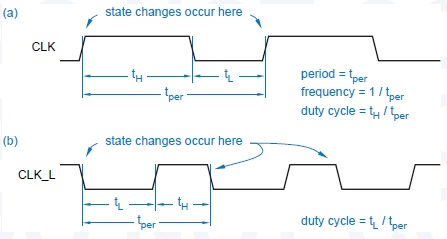
\includegraphics[width=5in]{reloj.jpg}
\caption{Señales de Reloj (a) Activo en alto (b) Activo en bajo}
\label{fig13}
\end{figure}


\section{Tabla de estado y diagrama de estado}

En la figura \ref{fig39} se muestra un ejemplo de tabla de estado, como se puede observar son tres tablas, cada tabla esta formado por tres columnas, en la primera tabla se muestra el estado actual (estado), en la segunda y tercera columna se muestran el estado siguiente y la salida separados por comas. Así por ejemplo en la tercera fila el estado actual es $a$, en la segunda columna el estado siguiente es $b$ cuando la señal de entrada $Y=0$ y la señal de salida es $0$, en el caso de que la señal de entrada sea $Y=1$ el estado siguiente sería $c$ y nuevamente la señal de salida será $0$.

\begin{figure}
\centering
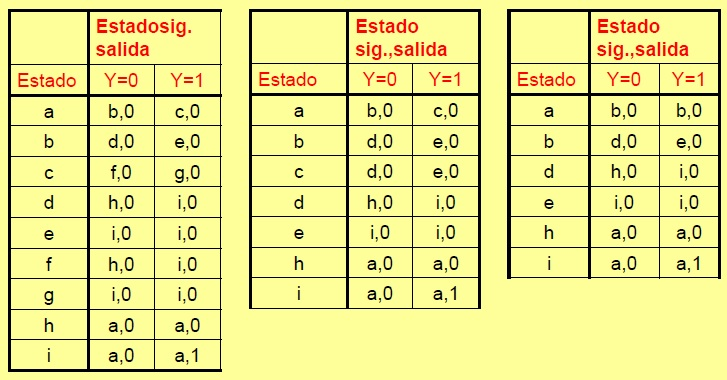
\includegraphics[width=5in]{TablaEstado.jpg}
\caption{Tabla de Estado del Ejemplo}
\label{fig39}
\end{figure}

Si analizamos la última fila de la primera tabla (la más grande), el estado actual sería el estado $i$ y el estado siguiente depende del valor se la variable de entrada, cuando $Y=0$ el estado siguiente es $a$ y la señal de salida es $0$ pero cuando $Y=1$ el estado siguiente es $a$ nuevamente y la señal de salida es $1$.

Entre la primera tabla y la tabla de en medio se realizó una reducción de estados. Esta reducción es posible cuando dos estados actuales con nombre diferentes tienen los mismos estados siguientes y las mismas señales de salida cuando las señales de entrada son las mismas, es decir la única diferencia entre dos renglones de la tabla de estados es el nombre del estado actual, así por ejemplo en la primera tabla el estado $d$ y el estado $f$ son equivalentes, y el estado $e$ y $g$ tambien son equivalente por lo cual pueden reducirse a uno solo, quedando como la tabla de estado de en medio. En la tabla de estado de en medio el estado $b$ y $c$ son equivalentes reduciéndose en la tabla de la izquierda que es la mas pequeña y simplificada.


En la figura \ref{fig40} se muestra un diagrama de estado de ejemplo, en estos diagramas los círculos representan los estado y dentro se ponen los nombres de los estados, las transiciones se representan por flechas en donde en la parte central se colocan las señales de entrada que provocan la transición separados por una diagonal de las señales de salida para esa transición.

\begin{figure}
\centering
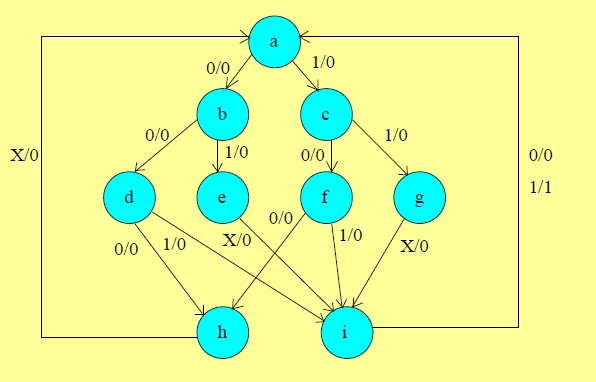
\includegraphics[width=5in]{DiagramaEstado.jpg}
\caption{Diagrama de Estado del Ejemplo}
\label{fig40}
\end{figure}

El número de flechas que salen de un estado depende del numero de señales de entrada, de tal forma si $n$ es el número de señales de entrada entonces el número de flechas que salen son $2^n$.

Por ejemplo, para el diagrama de estado de la figura \ref{fig40} el estado $d$ tiene dos flechas de salida (transiciones de salida) en donde cuando la señal de entrada es $1$ el estado siguiente es $i$ y la salida es $0$ y cuando la señal de entrada es $0$ el estado siguiente es $h$ y la señal de salida es $0$ también.

El diagrama de estado de la figura \ref{fig40} es equivalente a la tabla de estado mas pequeña (la de la izquierda)de la figura \ref{fig39}.

 
\section{Carta ASM}

\subsection{Representación de Estados}

El estado de una máquina de estados es la memoria de la historia pasada, suficiente para
determinar las condiciones futuras. En la siguiente figura se muestra la representación del estado.
Un estado se representa con un rectángulo y con su nombre simbólico en el extremo superior,
encerrado en un círculo.


\begin{figure}
\centering
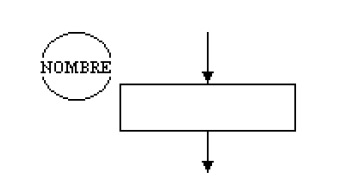
\includegraphics[width=3in]{ASMestado.jpg}
\caption{Representación de estado en carta ASM}
\label{fig14}
\end{figure}

\subsection{Representación de decisiones }

Las decisiones permiten seleccionar el camino que el algoritmo de la máquina de estados debe
tomar de acuerdo a la variable o variables de entrada evaluadas. Las decisiones se representan
mediante un rombo con el nombre de la variable a probar o una función que evalúe varias variables.

\begin{figure}
\centering
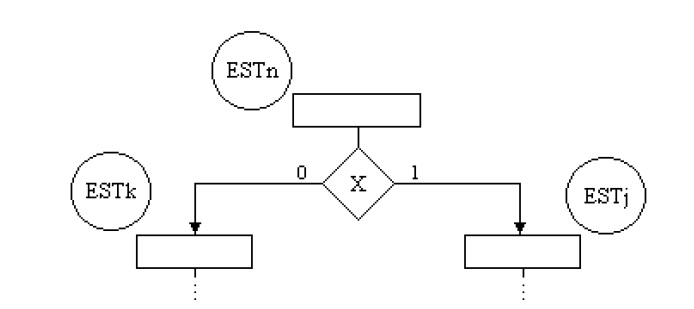
\includegraphics[width=4in]{ASMdecisiones.jpg}
\caption{Representación de decisiones en carta ASM}
\label{fig15}
\end{figure}

\subsection{Representación de Salidas}

Salidas no condicionales. Sirven para indicar la activación de una variable de salida. Para
representarlas, se escriben dentro del rectángulo de estado, los nombres de las variables de salida
que se activan en ese estado. Las salidas no condicionales no dependen de las condiciones de
entrada, sólo dependen del estado actual. La figura \ref{fig16} muestra la activación de las salidas VAR1 y
VAR2 en el estado EST1.

\begin{figure}
\centering
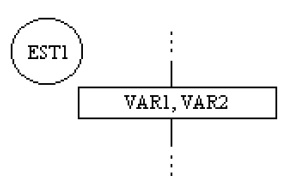
\includegraphics[width=2.5in]{ASMnocondicional.jpg}
\caption{Representación de las salidas no condicionales en carta ASM}
\label{fig16}
\end{figure}

\subsection{Salidas Condicionales}

Estas salidas se presentan solamente cuando ciertas condiciones de
entrada existen. Se representan con un óvalo y los nombres de las salidas dentro de él.

\begin{figure}
\centering
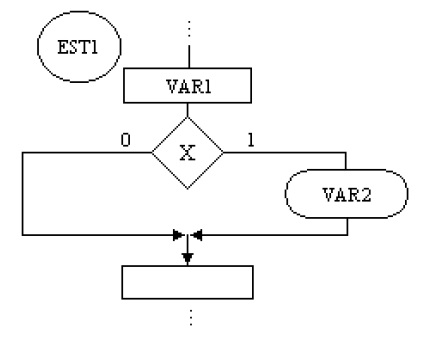
\includegraphics[width=3in]{ASMcondicional.jpg}
\caption{Representación de las salidas condicionales en carta ASM}
\label{fig17}
\end{figure}

Para este ejemplo, si en el estado EST1 la variable de entrada X vale uno, entonces las salidas
VAR1 y VAR2 serán activadas. Si X es igual a cero solamente se activará VAR1.

\section{Ejemplo de Cartas ASM}

A continuación se presentan algunos ejemplos para aclarar las ideas antes expuestas.

\begin{itemize}
\item Diseñe un dispositivo que genere cierta secuencia binaria sólo cuando la variable INICIO sea
igual a uno. Además esta secuencia dependerá del valor de la entrada X. Si X=0 la secuencia binaria que se genera es la siguiente: 11, 10, 01, por el contrario, si X=1 la secuencia es: 01,
10, 11. Considere que cada pareja binaria se genera con un ciclo de reloj de diferencia.

\end{itemize}
\subsubsection{Ejemplo 1}
Cuando se hace el diseño digital de un sistema es necesario hacer un diagrama de bloques que
clarifique cuáles son las señales de entrada, cuáles las señales de salida, quién es el controlador y
qué se está controlando.

Para este ejemplo, las señales de entrada son INICIO y X, y las señales de salida son las que
representan la secuencia que se quiere generar, nombrémoslas VAR1 y VAR0.

El diagrama de bloques queda de la siguiente manera.

\begin{figure}
\centering
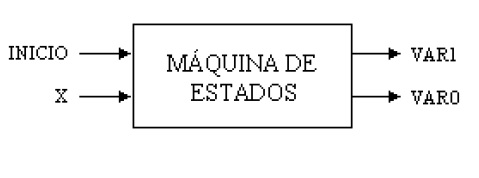
\includegraphics[width=3in]{EjemploMaquina1.jpg}
\caption{Diagrama de bloque del ejemplo 1}
\label{fig18}
\end{figure}

Y la carta ASM para esta máquina de estados se muestra en la figura \ref{fig19}

\begin{figure}
\centering
\includegraphics[width=3in]{ASMEjemplo1.jpg}
\caption{Carta ASM del ejemplo 1}
\label{fig19}
\end{figure}

De la figura \ref{fig19} se puede observar que para activar una señal de salida incondicional, en un
estado en particular, es necesario colocar su nombre dentro del rectángulo del estado.

\subsubsection{Ejemplo 2}

\begin{itemize}
\item Convertir el siguiente código en lenguaje ‘C’ a una carta ASM.

\begin{verbatim}
for (x=a; x<=b; x=x+c) {
     var1 = 1;
     var2 = 0;
}
var1=0;

\end{verbatim}
\end{itemize}





\begin{figure}
\centering
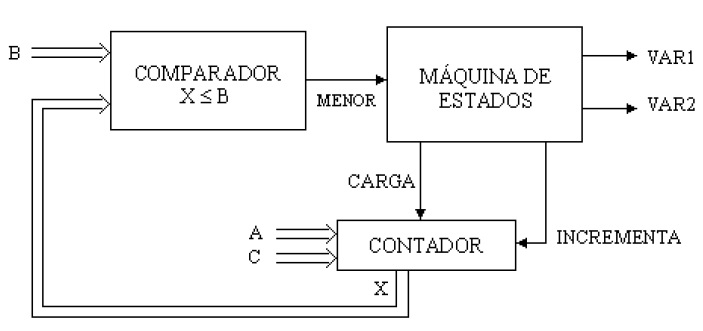
\includegraphics[width=3in]{bloquesejemplo1b.jpg}
\caption{Diagrama de bloques  del ejemplo 2}
\label{fig20}
\end{figure}

Se utiliza un contador para cargar el valor inicial de X o incrementar su valor en C unidades. La
activación de la señal CARGA inicializará el valor de $X$ con $A$, mientras que la activación de la
señal INCREMENTA incrementará el valor de $X$ en $C$ unidades. También se cuenta con un
comparador que evalúa la condición $X <= B$. Si $X$ es menor o igual a $B$, el resultado es la activación
de la señal MENOR, en caso contrario, la señal MENOR permanece en cero.
El algoritmo de la máquina de estados es el siguiente.

\begin{figure}
\centering
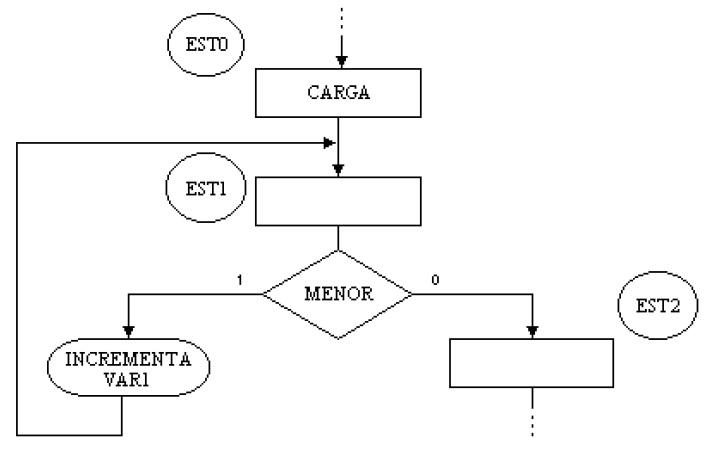
\includegraphics[width=3in]{ASMejemplo2.jpg}
\caption{Carta ASM  del ejemplo 2}
\label{fig21}
\end{figure}

En el estado EST0 se activa la señal CARGA con el fin de cargar en el contador el valor inicial
de X. En el estado EST1 se pregunta por la variable de entrada MENOR, si esta es igual a cero, la
condicion X . B es falsa. Si MENOR es igual a uno, la condicion es verdadera y por tanto, son
activadas las senales INCREMENTA y VAR1 como salidas condicionales.

\subsubsection{Ejemplo 3}

Convertir el siguiente código en lenguaje ‘C’ a una carta ASM
\begin{verbatim}
while( x==0 ) {
   var5 = 1;
   var2 = 1;
   if( z==0 ) {
        x = 1;
        var5 = 0;
   }
}
var5 = 0;
var2 = 0;
\end{verbatim}

El valor de la variable X puede ser modificado por la lógica externa o por la
máquina de estados. Por ello, para representar a X, utilizaremos un flip-flop cuyo valor será puesto a uno ó a cero dependiendo de las señales internas y externas.

El diagrama de bloques de este sistema es el siguiente (ver figura \ref{fig22}).

\begin{figure}
\centering
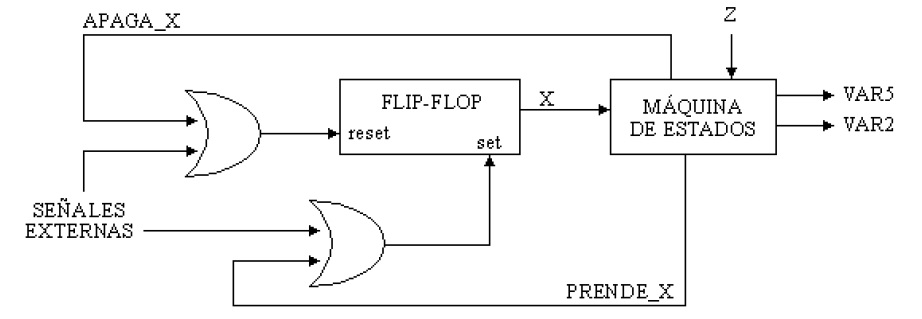
\includegraphics[width=4in]{ASMbloques3.jpg}
\caption{Diagrama de bloques  del ejemplo 3}
\label{fig22}
\end{figure}

Y el algoritmo de la máquina de estados se muestra en la figura \ref{fig23}.

\begin{figure}
\centering
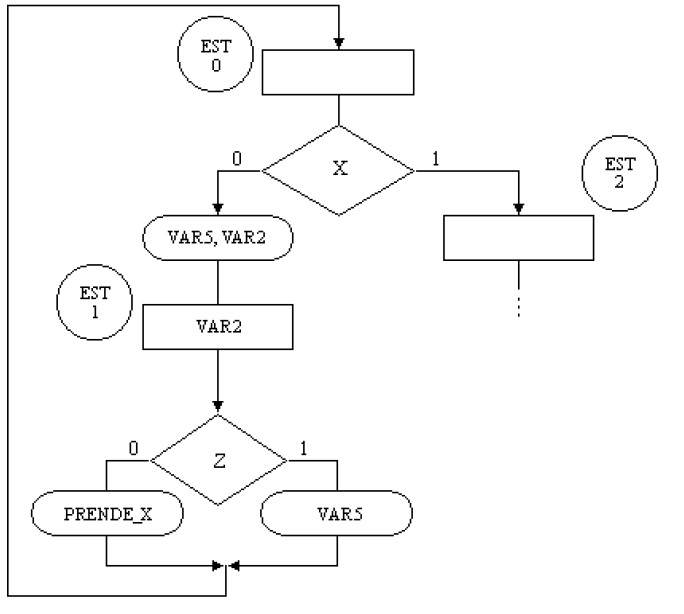
\includegraphics[width=4in]{ASMejemplo3.jpg}
\caption{Carta ASM  del ejemplo 3}
\label{fig23}
\end{figure}




\subsubsection{Ejemplo 4}

Convertir el siguiente código en lenguaje ‘C’ a una carta ASM.
\begin{verbatim}
if ( x==n ) {
    var1 = 1; var2 = 0;
} 
else {
    var1 = 0; var2 = 1;
}
var1 = 0;
var2 = 0;

\end{verbatim}

En este ejemplo las variables de entrada x y n están definidas como variables de un sólo bit. Para
hacer la comparación de las variables x y n se usa la función lógica XOR, que valdrá cero cuando x
y n sean iguales, y uno, cuando sean diferentes (ver figura \ref{fig24}).

\begin{figure}
\centering
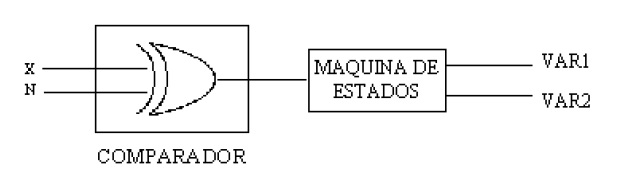
\includegraphics[width=4in]{ASMbloque4.jpg}
\caption{Diagrama de bloques  del ejemplo 4}
\label{fig24}
\end{figure}

Y el algoritmo de esta máquina de estados se muestra en la figura \ref{fig25}.

\begin{figure}
\centering
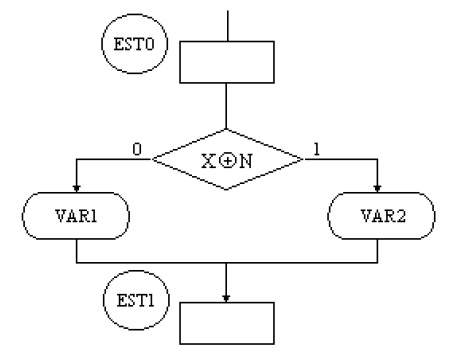
\includegraphics[width=4in]{ASMejemplo4.jpg}
\caption{Carta ASM  del ejemplo 4}
\label{fig25}
\end{figure}


En el diagrama de la figura \ref{fig25} se observa que si deseamos activar una señal de salida condicional, en un estado
en particular, es necesario colocar su nombre dentro de un óvalo

\subsubsection{Ejemplo 5}

\begin{itemize}
\item Usando un diagrama de tiempos mostrar la diferencia entre las cartas ASM de la figura 2.15, en donde la variable de salida VAR2 está como salida condicional en la carta ASM1 y como salida incondicional en la carta ASM2.
\end{itemize}

\begin{figure}
\centering
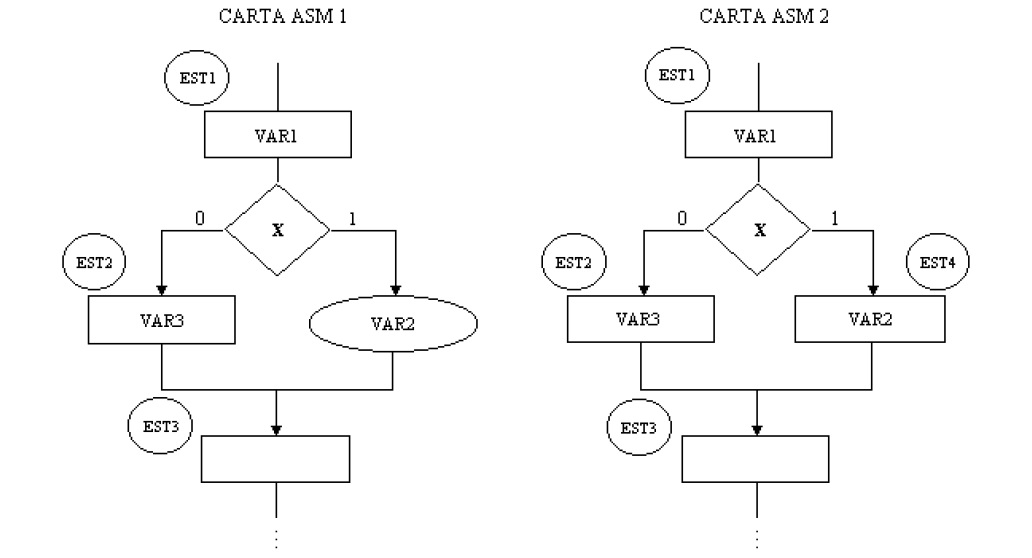
\includegraphics[width=4in]{ASMejemplo5.jpg}
\caption{La salida VAR2 en la carta ASM1 se presenta como salida condicional, mientras que en la carta ASM2 se presenta como no condicional.}
\label{fig26}
\end{figure}

Si observa detenidamente el diagrama de tiempos de la figura \ref{fig28} observará que la diferencia principal entre las dos cartas ASM es el tiempo cuando se activa la salida VAR2. Cuando está como salida condicional se activa en el estado EST1 junto con VAR1, y cuando está como salida incondicional se activa un flanco positivo después que VAR1.



\begin{figure}
\centering
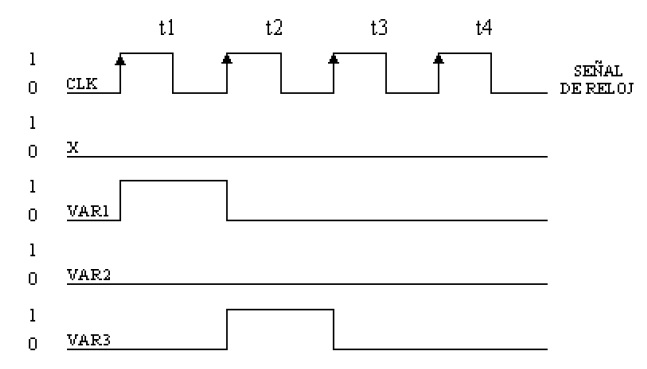
\includegraphics[width=3.5in]{ASMtiempos1.jpg}
\caption{Diagrama de tiempos para las cartas ASM1 y ASM2, con x=0.}
\label{fig27}
\end{figure}

A continuación se muestra el diagrama de tiempos para la carta ASM1 cuando la entrada X es
igual que cero. Este diagrama de tiempos es idéntico para la carta ASM2.

\begin{figure}
\centering
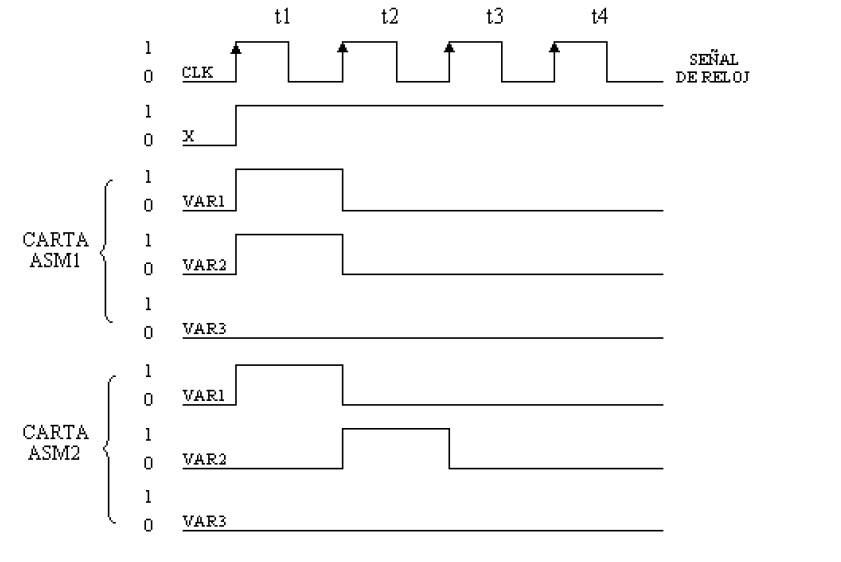
\includegraphics[width=3.5in]{ASMtiempos2.jpg}
\caption{Diagrama de tiempos para las cartas ASM1 y ASM2, con x=1.}
\label{fig28}
\end{figure}

A continuación se muestran los diagramas de tiempos cuando X es igual a 1.



\chapter{Estructura Básica de Una computadora}

En este capítulo se diseñarán algunos de los componentes que integran una computadora. En la
figura \ref{fig29} se muestra el diagrama de bloques general de una computadora.

\begin{figure}
\centering
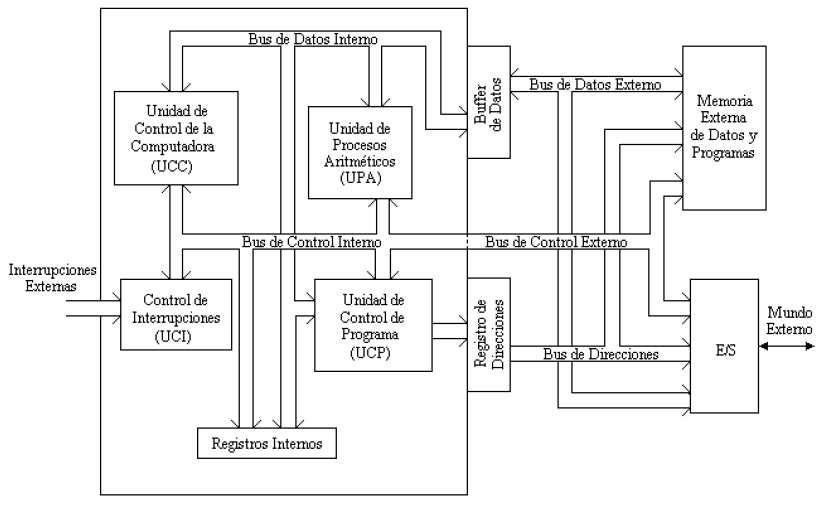
\includegraphics[width=5in]{computerbasica.jpg}
\caption{Estructura básica de una computadora.}
\label{fig29}
\end{figure}

Como se observa en el diagrama de bloques, una computadora está constituida internamente por
cinco bloques básicos:

\begin{itemize}
\item Unidad de Control de la Computadora (UCC). Se encarga de enviar las señales de control a
los demás elementos de la computadora.
\item Unidad de Procesos Aritméticos (UPA). En ella se realizan todas las operaciones lógico
aritméticas.
\item Unidad de Control de Programa (UCP). Calcula la dirección de la siguiente instrucción a ser
ejecutada.
\item Unidad de Registros Internos. Conjunto de registros capaces de almacenar información.
\item Unidad de Control de Interrupciones (UCI). Se encarga del manejo de las interrupciones
externas.
\end{itemize}

A continuación se describe cada uno de estos componentes.

\section{Unidad de Control de la Computadora (UCC)}

La UCC se encarga de decodificar las instrucciones en ensamblador y de ejecutar las microoperaciones
necesarias (representadas por medio de cartas ASM) para llevarlas a cabo. Esto es, por
cada instrucción en lenguaje ensamblador, serán activadas secuencialmente una serie de señales que
le indican a los diferentes componentes de la arquitectura la operación a realizar. La parte
fundamental de la UCC es el secuenciador, como se muestra en la figura \ref{fig30}

\begin{figure}
\centering
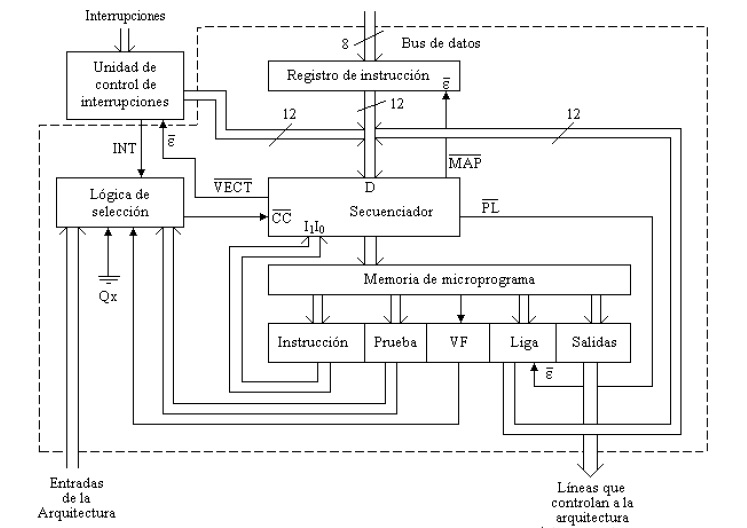
\includegraphics[width=5in]{UCC.jpg}
\caption{Unidad de control de la computadora (UCC)}
\label{fig30}
\end{figure}

La dirección de salto en la entrada D del secuenciador puede
venir de tres lugares diferentes: del registro de instrucción, de la unidad de control de interrupciones,
ó del campo de liga de la memoria de microprograma. La figura \ref{fig30} ilustra esta configuración.
El tamaño de la palabra de las instrucciones codificadas es de 8 bits. Este número es cargado en
el registro de instrucciones y extendido de 8 a 12 bits mediante la adición de cuatro ceros a la derecha. Este nuevo valor es la dirección en la memoria de microprograma en donde comienzan las
micro-operaciones que ejecuta esta instrucción.
En el campo de salidas de la memoria de microprograma se tienen las líneas que controlan tanto a
la arquitectura interna como a la externa, las cuales se activan según la instrucción a ejecutar.
Por otra parte, las entradas de la arquitectura indican el estado en el que se encuentra tanto la
arquitectura interna como la externa, y sirven para que el secuenciador pueda tomar decisiones de
acuerdo a ciertos criterios. Estas entradas son seleccionadas en el bloque de lógica de selección por
medio del campo de prueba. La línea de INT también se conecta a la lógica de selección para revisar
si existe alguna petición de interrupción.
Otra forma alternativa de diseñar la UCC es utilizando los lenguajes de descripción de hardware
como Verilog HDL, VHDL ó AHDL. Utilizando alguno de estos lenguajes y el código de la
instrucción que se desea ejecutar, es posible describir los pasos requeridos para ejecutar dicha
instrucción.

\section{Unidad de Procesos Aritméticos(UPA)}


La unidad de procesos aritméticos (UPA) se encarga de realizar las operaciones lógico
aritméticas básicas. Para ello, cuenta con una unidad lógico aritmética que le permite hacer sumas,
restas, y operaciones lógicas AND, OR exclusiva, OR exclusiva negada, entre otras. La UPA
también cuenta con un registro de corrimiento auxiliar para guardar valores intermedios que
posteriormente operará.
La figura \ref{fig31} muestra una UPA de ocho bits basada en una UPA fabricada por AMD de cuatro
bits (D2901). Este dispositivo, como en el caso del secuenciador, no existen físicamente en la
actualidad, sino como un módulo en software que puede ser integrado en un sistema digital.


\begin{figure}
\centering
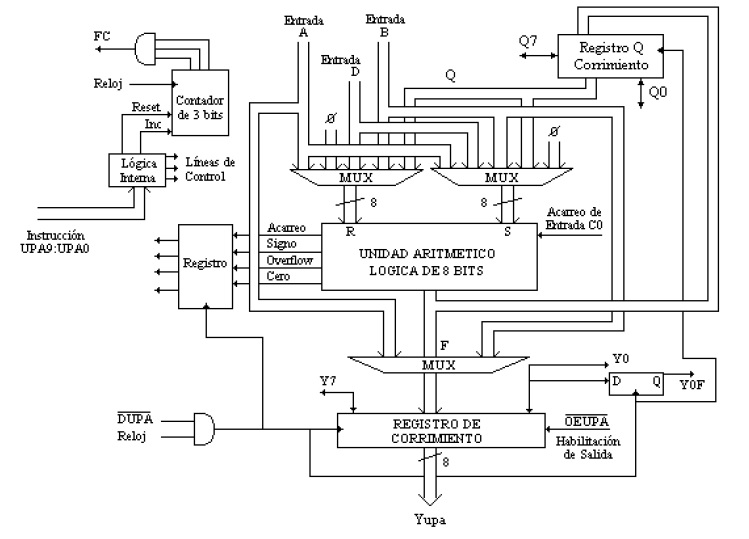
\includegraphics[width=4in]{ALU.jpg}
\caption{Diagrama de bloques de la unidad de procesos aritméticos (UPA)}
\label{fig31}
\end{figure}


Como se observa en la figura \ref{fig31}, las fuentes de la unidad lógico aritmética pueden venir de
cinco lugares diferentes: de la entrada A, de la entrada B, del registro de corrimiento auxiliar Q, de
la entrada de datos D y el valor de cero.
El resultado de la operación de la ALU puede ser desplazado a la derecha o a la izquierda antes
de ser guardado en alguno de los registros de destino. Estos registros de destino son el registro de
corrimiento Yupa y el registro de corrimiento Q. Además, observe que la señal DUPA habilita o no
la carga de un resultado o de un corrimiento en los registros de destino.
El diagrama de bloques de la UPA se muestra a continuación.


\begin{figure}
\centering
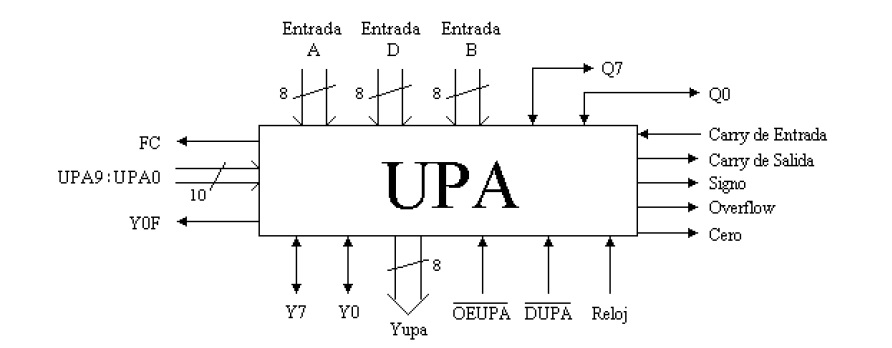
\includegraphics[width=4in]{ALU2.jpg}
\caption{Unidad de procesos aritméticos (UPA)}
\label{fig32}
\end{figure}

Las figuras \ref{fig33}, \ref{fig34} y \ref{fig35} muestran la relación existente entre las líneas de control de la UPA
(UPA9:UPA0) y las operaciones que ésta puede ejecutar.

En particular, la figura \ref{fig33} presenta la selección de las fuentes de la ALU, la figura \ref{fig34} las
operaciones que ejecuta la ALU, y la figura \ref{fig35} los destinos y desplazamientos del resultado
obtenido por la ALU


\begin{figure}
\centering
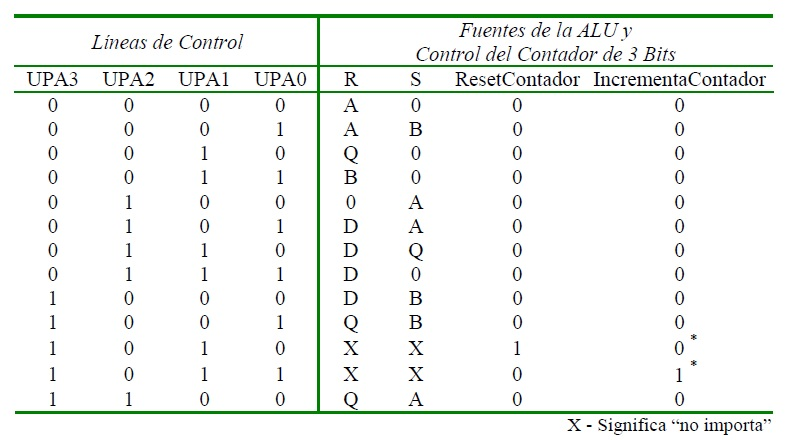
\includegraphics[width=4in]{tabla1.jpg}
\caption{Selección de las fuentes de la ALU y líneas de control para el contador de 3 bits.}
\label{fig33}
\end{figure}


\begin{figure}
\centering
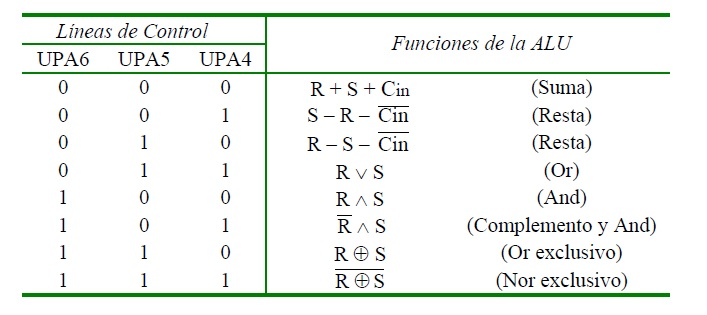
\includegraphics[width=4in]{tabla2.jpg}
\caption{Operaciones de la ALU}
\label{fig34}
\end{figure}

\begin{figure}
\centering
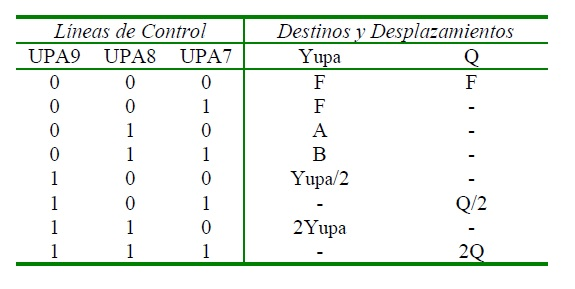
\includegraphics[width=4in]{tabla3.jpg}
\caption{Destinos y desplazamientos de la UPA}
\label{fig35}
\end{figure}

Por ejemplo, para realizar la operación lógica OR entre las entradas A y B, y colocar el resultado
en el registro Yupa, se necesitan activar las siguientes líneas.
\begin{itemize}
\item  Las fuentes A y B se seleccionan con UPA3 UPA2 UPA1 UPA0 = 0001
\item La función OR se selecciona con las líneas UPA6 UPA5 UPA4 = 011
\item El destino Yupa se selecciona con las líneas UPA9 UPA8 UPA7 = 000
\end{itemize}

La siguiente figura muestra la activación de las señales de control de la UPA para efectuar la
operación $Yupa=A \vee B$ usando cartas ASM.

\begin{figure}
\centering
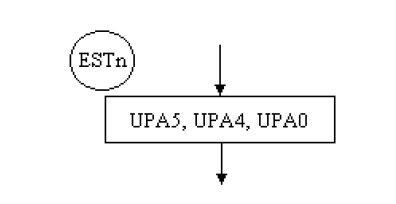
\includegraphics[width=3in]{tabla4.jpg}
\caption{Activación de las líneas de control en una carta ASM.}
\label{fig36}
\end{figure}

La UPA también tiene unas líneas de salida que reflejan el resultado de la última operación hecha
por la ALU. La línea Z indica si el resultado fue cero; SIGNO indica el valor del bit más
significativo; y OVR indica si hubo sobreflujo. También se cuenta con dos líneas de acarreo: uno de
entrada y otro de salida.

\section{Registros Internos}

La computadora requiere una serie de registros que tanto el
usuario como el CPU pueden utilizar. Los registros, denominados acumuladores, sirven
únicamente como dispositivos de almacenamiento. Los registros, denominados registros
contadores, tienen mayor funcionalidad, pues además de servir como dispositivos de
almacenamiento, permiten incrementar o decrementar el dato guardado.

\section{Unidad de control de Programa (UCP)}

La UCP se encarga de calcular la dirección de memoria en donde se encuentra el código de la
siguiente instrucción a ejecutar. Para esto, cuenta con un registro denominado contador de programa
(PC) que contiene la dirección de la siguiente instrucción a ejecutar, y de un registro llamado
apuntador de pila (AP) que apunta a una memoria en donde se guardan las direcciones de regreso de
las llamadas a subrutinas. La figura \ref{fig37} muestra el diagrama de bloques de la UCP

\begin{figure}
\centering
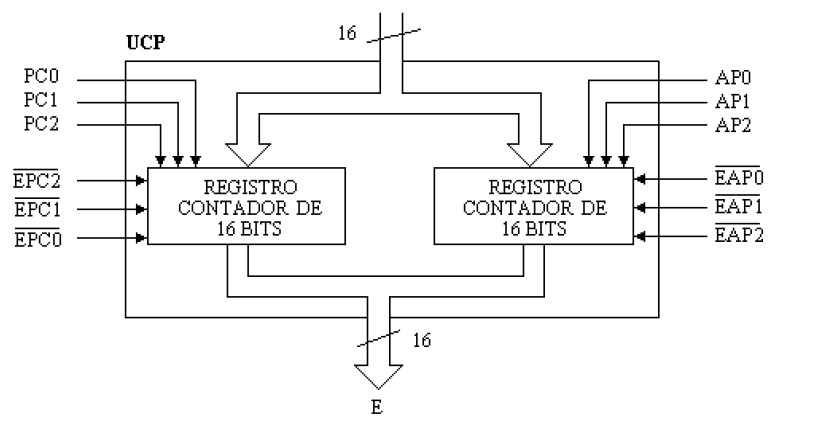
\includegraphics[width=3in]{UCP.jpg}
\caption{Unidad de control de programa (UCP)}
\label{fig37}
\end{figure}


\section{Unidad de Control de Interrupciones (UCI)}

La UCI se encarga de recibir peticiones de interrupciones externas. Tales peticiones provienen de
alguno de los dispositivos conectados a las líneas IRQ y XIRQ . Como respuesta, la UCI envía una
dirección de salto al secuenciador indicándole el inicio del algoritmo de máquina de estados que
atiende la interrupción pedida.
Antes de atender la interrupción, el algoritmo de la máquina de estados guarda en la pila la
dirección de la siguiente instrucción a ser ejecutada, dirección que está contenida en el registro PC.
Los valores de los acumuladores, de los registros X e Y, y del registro de estados, también son
guardados en la pila. Una vez guardados estos datos, el contador de programa (PC) se carga con la
dirección de inicio de la rutina de atención a la interrupción. En el capítulo siguiente se muestran las
cartas ASM que atienden las interrupciones. En la figura \ref{fig38} se muestra el diagrama de bloques de una UCI.



\begin{figure}
\centering
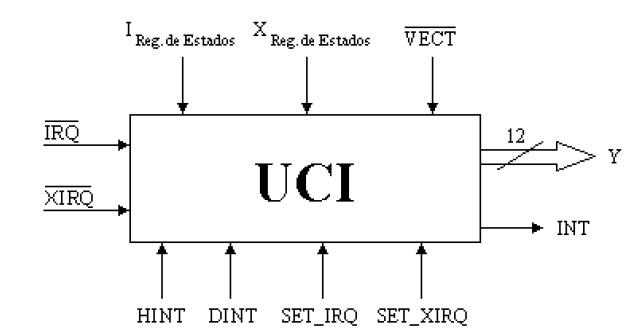
\includegraphics[width=3in]{UCI.jpg}
\caption{Diagramas de bloques externo de la UCI}
\label{fig38}
\end{figure}






\chapter{Memoria}
En este capítulo buscaremos analizar los principios de funcionamiento de las memorias, clasificarlas y estudiarlas conectadas a un microprocesador.

\section{Principios de funcionamiento}

\subsection{Multivibradores biestables con transistores}

Supongamos tener el circuito de la Fig. \ref{fig5}. En dicho circuito admitiremos que todos los elementos conectados a cada transistor, son exactamente iguales a sus equivalentes conectados sobre el otro. Por su parte, ambos transistores tendrán exactamente las mismas características estáticas y dinámicas.

\begin{figure}
\centering
\includegraphics[width=5in]{Biestable.jpg}
\caption{Diagrama Básico de un flip flop con transistores}
\label{fig5}
\end{figure}

En tales circunstancias, $I_{C1} = I_{C2}$, $I_{B1} = I_{B2}$ y $V_{CE1} = V_{CE2}$.
Este sistema es absolutamente simétrico, pero, como veremos a continuación inestable.

Supongamos que por alguna eventualidad, la corriente de colector del transistor $Q_{1}$ aumenta en forma diferencial. Ello producirá un aumento en la tensión sobre el resistor $R_1$, disminuyendo por aplicación de la segunda regla de Kirchoff $V_{CE1}$. Esta disminución produce una disminución en la corriente de base del segundo transistor, que produce una disminución en $I_{C2}$, lo que produce una disminución en la tensión sobre $R_2$ y aumento en la tensión $V_{CE2}$. Este aumento genera un incremento en la corriente de base del transistor 1 que a su vez lleva a que $I_{C1}$ crece, lo que fue nuestro punto de partida. Simbólicamente:

\begin{figure}
\centering
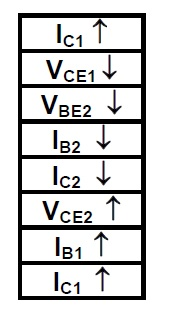
\includegraphics[width=1.5in]{biestable2.jpg}
\caption{Evolución del circuito del biestable con transistores al cambiar alguna de sus variables.}
\label{fig6}
\end{figure}

El hecho que al aumentar una magnitud eléctrica ($I_{C1}$ en nuestro ejemplo, pero podría haber sido cualquier otra), el sistema refuerza este aumento, se describe diciendo que se trata de un circuito con realimentación positiva.
Esta realimentación culminará llevando a $Q_1$ a la saturación mientras que $Q_2$ terminará cortado.
Este circuito permanecerá en este estado estable hasta que un pulso negativo1 en el colector del transistor cortado o un pulso positivo en el transistor saturado invierta el estado de conducción de ambos transistores. En este nuevo estado el circuito permanecerá hasta que por medio de otra señal externa se vuelvan a cambiar los estados.
Esto nos lleva a proclamar que el sistema tiene dos estados estables y se trata de un circuito multivibrador biestable.


\section{Almacenamiento de información binaria}

Supongamos que deseamos almacenar información binaria para su posterior empleo. Supongamos que deseamos almacenar 16 bits de información. Según una regla empírica de mejor aprovechamiento del área del circuito integrado, se buscará que la configuración de la memoria sea cuadrada, es decir que tenga la misma cantidad de filas que de columnas .


\begin{figure}
\centering
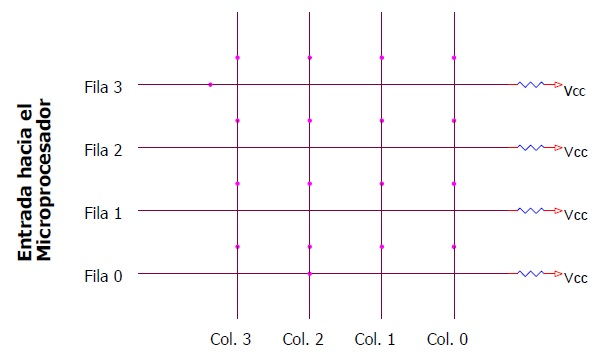
\includegraphics[width=5in]{entrada.jpg}
\caption{Esquema inicial de una memoria}
\label{fig7}
\end{figure}

Analicemos el esquema de la Fig. \ref{fig7}. Si desde el microprocesador leemos las líneas de entradas allí indicadas, se obtendrá en todo momento \grqq 1 \grqq en todas las filas. Ello es debido a que al no existir otra conexión, las resistencias de pull up cumplirán su cometido forzando \grqq 1 \grqq lógico en todas las entradas.

\begin{figure}
\centering
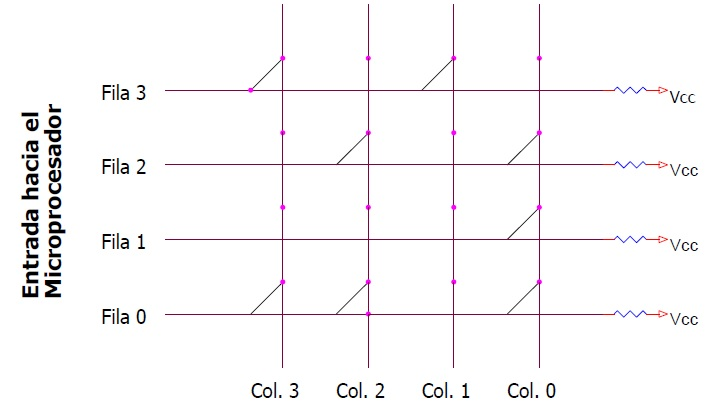
\includegraphics[width=5in]{entrada2.jpg}
\caption{Esquema de una memoria básica con información}
\label{fig8}
\end{figure}

En la Fig. \ref{fig8} se observa un esquema similar al de Fig. \ref{fig7}, con el agregado de bits de información por medio de conexiones entre filas y columnas.
Supongamos que colocamos un \grqq 0 \grqq lógico en una de las columnas y \grqq 1 \grqq  lógico en todas las demás columnas. Como ejemplo, colocamos \grqq 0 \grqq en la columna 3. Ese \grqq 0\grqq aparecerá en las filas 3 y 0, mientras que las filas 2 y 1 quedarán fijas a \grqq 1 \grqq por los resistores de pull-up.
Bajo esta idea, podremos colocar un decodificador con salidas activas bajas que seleccione una de las columnas, mientras que las demás permanecerán en \grqq 1 \grqq . Podremos \grqq soldar \grqq conductores entre filas y columnas para forzar \grqq 0 \grqq en esa posición de memoria.
Esta idea es bastante primitiva ya que para modificar el contenido de una posición de memoria deberemos \grqq soldar \grqq y \grqq desoldar \grqq conductores en las intersecciones de fila y columna.
Por otro lado, el bosquejo de la Fig. \ref{fig8} presenta un inconveniente insalvable que la presencia de conexiones \grqq fantasmas \grqq . Supongamos colocar un \grqq 0 \grqq en la columna 2. Ello producirá que leamos dicho \grqq 0 \grqq en las filas 0 y 2 como fue nuestro objetivo al conectar dichas filas y columnas.

Ahora bien, como producto de las uniones ohmicas de la columna 2 con la fila 0, dicha fila se hallará a potencial del estado lógico \grqq 0 \grqq. Por la unión entre fila 0 y columna 3, toda la columna 3 se hallará a potencial del \grqq 0 \grqq y por ende, se leerá \grqq 0 \grqq en la fila 3, lo cual es un error pues sobre la columna 2 no existe unión con la fila 3. Ese valor leído es erróneo y es lo que se denomina conexión fantasma y es producido por el error de implementar los ceros lógicos con uniones puramente óhmicas entre fila y columna.

\begin{figure}
\centering
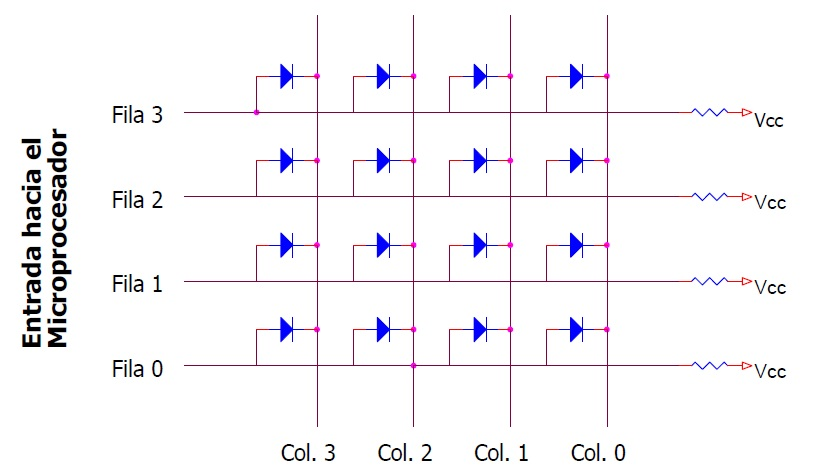
\includegraphics[width=5in]{entrada3.jpg}
\caption{Esquema de una memoria mejorada con diodos}
\label{fig9}
\end{figure}

Una posible solución consiste en colocar diodos en lugar de conductores en las uniones como se observa en la Fig. \ref{fig9}. De esa forma, el \grqq 0 \grqq lógico forzado por el decodificador en una columna, aparecerá en las filas en las que se hallen los diodos conectados, pero todos los demás diodos quedarán polarizados en inversa por lo que no se producirán conexiones fantasmas.
Seguimos manteniendo la limitación que consiste en que para modificar el contenido de una posición de memoria deberán desoldarse y resoldarse diodos.
La mejor alternativa para dar flexibilidad a la memoria y poder modificar el contenido de la misma, consiste en conectar transistores NPN o MOS en las uniones, con el emisor apuntando hacia lo que antes era el cátodo de los diodos, como se aprecia en la Fig. 5. Esos transistores pueden ser uno de los transistores del flip-flop de la Fig. \ref{fig5}, de forma que pueda cambiarse el contenido de cada posición de memoria cambiando el estado de cada biestable.
En el ejemplo que estamos analizando, se necesitarán 16 biestables ya que se conectará uno en cada intersección de fila y columna. Cada biestable mantendrá la vinculación entre fila y columna hasta que se modifique su estado y mientras se mantenga la alimentación del sistema.
Debe tenerse en cuenta que existirá un circuito adicional (ni dibujado ni analizado aquí para no complicar innecesariamente el esquema) que será el encargado de modificar el estado de los biestables según la información que se desee guardar.
En la Fig. 5, se observa también la aparición de un decodificador con habilitación /CS, que permite seleccionar una columna al aparecer una determinada dirección. También se observa un amplificador separador (buffer tristate) que permitirá volcar el contenido de una posición de memoria (seleccionada por el decodificador) sobre el bus de datos del microprocesador, cuando la señal /OE lo permita.

\begin{figure}
\centering
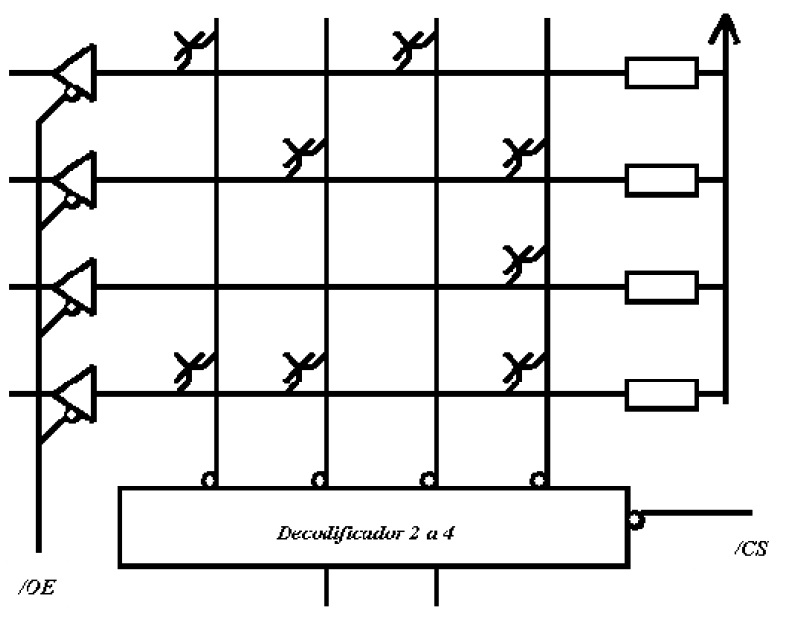
\includegraphics[width=5in]{entrada4.jpg}
\caption{Bosquejo de una memoria elemental}
\label{fig10}
\end{figure}

\chapter{Una breve historia de la Arquitectura \emph{ARM}}
La compañía ARM se formo en 1990 como \emph{Advanced RISC Machines Ltd} una empresa formada por Apple Computer, Acorn Computer Group, y VLSI Technology. En 1991, ARM introduce la familia de procesadores ARM6, y VLSI se convierte en la primera compañia a quien se le da la licencia de fabricación. Posteriormente, otras compañias, incluyendo Texas Instrument, NEC, Sharp, y ST Microelectronics, solicitaron licencias de fabricación de los diseños ARM, extendiendo las aplicaciones de los procesadores ARM hacia los telefonos móviles, discos duros de computadoras, asistentes personales (PDA), sistemas de entretenimiento en casas, y muchos otros productos de consumo.
Hoy en día, los socios de ARM envían mas de 2 mil millones de procesadores ARM cada año. A diferencia de muchas empresas de semiconductores, ARM no fabrica procesadores o vende directamente los chips. En cambio, ARM licencia los diseños de procesadores a los socios de negocio, incluyendo la mayoría de las compañías de semiconductores más importantes del mundo. Basados en los procesadores diseñados por ARM de bajo costo y eficiencia energética, estos socios ran sus procesadores, microcontroladores, y soluciones SoC (\emph{System on Chip}). Su modelo de negocios se llama comúnmente Licenciamiento de Propiedad Intelectual (\emph{intellectual property IP})

\section{Versiones de la Arquitectura}

Conforme pasaron los años, ARM ha continuado desarrollando nuevos procesadores y bloques de sistemas. Estos incluyen el popular procesador \textbf{ARM7TDMI} y, mas recientemente, el procesador \textbf{ARM1176TZ(f)-S}, el cual es usado en aplicaciones de alta tecnología tales como los \emph{smartphones}.

ARM amplio su portafolio de productos diversificando su desarrollo de CPU, lo cual resultó en la arquitectura version 7 o v7. En esta versión, el diseño de la arquitectura esta dividida en tres perfiles (ver Figura \ref{fig1}):

\begin{itemize}
\item El perfil A (ARMv7-A): Es un procesador de aplicación el cual esta diseñado para manejar aplicaciones complejas tales como Sistemas Operativos Embebidos (OSs) (e.g. Symbian, Lynux, and Windows embebido). Estos procesadores requieren de alta potencia de procesamiento, soporte para sistema de memoria virtual con unidades de manejo de memoria (MMU), y opcionalmente, mejoramiento den el soporte de Java y ambientes de ejecución segura de programas.

\item Perfil R (ARMv7-R): Son procesadores de alto rendimiento, en tiempo real, específicamente diseñados para el mercado en tiempo real y aplicaciones de alto rendimiento. Aquellas aplicaciones, tales como sistemas de frenado de alta eficiencia y controladores de  discos duros, en los cuales altas potencias de procesamiento y gran confiabilidad son esenciales y por lo que bajos tiempos de espera son importantes.
\item Perfil M (ARMv7-M): Estos procesadores con para aplicaciones de bajo costo en los cuales  la eficiencia de procesamiento es importante así como los costos, el consumo de potencia, poco tiempo de espera de las interrupciones, fácil de usar así como aplicaciones de control industrial, incluyendo sistemas de control en tiempo real.

\end{itemize}

\begin{figure}
\centering
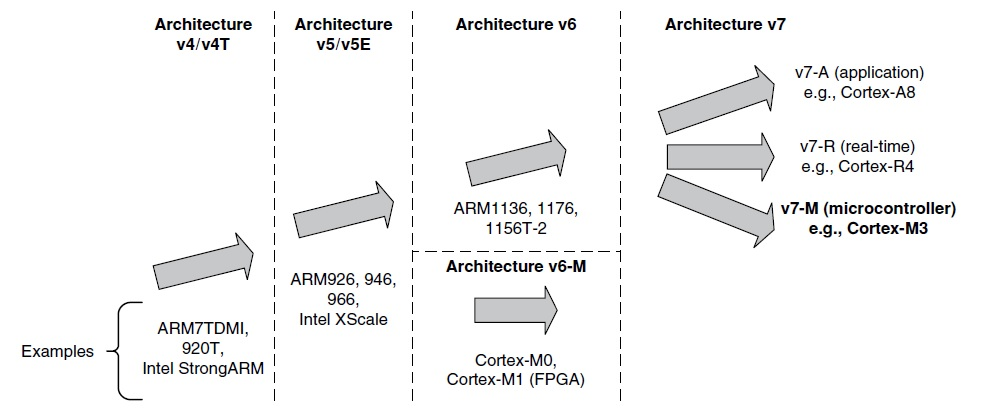
\includegraphics[width=5in]{HistoriaARM.jpg}
\caption{Evolución del la arquitectura de Procesadores ARM}
\label{fig1}
\end{figure}

\section{Nombres de los Procesadores}
A comienzos de los 1990, los sufijos fueron usados para indicar características de los procesadores. Por ejemplo, con el procesador ARM7TDMI, la T indica soporte de \emph{Thumb Instruction}, D indica \emph{JTAG debugging}, M indica \emph{fast multiplier}, y I indica \emph{embedded ICE module}. Sin embargo, los sufijos no fueron utilizados más en las nuevas familias de procesadores. En su lugar, variaciones en la interfaz de memoria, cache y memoria acoplada (TCM) crearon un nuevo esquema de nombramientos de los procesadores.
El procesador ARM con cache y MMU se le da ahora el sufijo "26", o el sufijo "36", donde el procesador con MPUs se les da el sufijo "46" (e.g. ARM946E-S). En adición, otros sufijos son anexados para indicar que tiene tecnología  sintetizable (S) o Jazelle (J). En la figura \ref{fig2}  se presenta un resumen de los nombres de procesadores. 


Con la versión 7 de la arquitectura, ARM ha migrado de este complejo que necesita ser decodificado, moviendose a un nombre consistente para la familia de procesadores, con cortex se inicio esta idea.

\begin{figure}
\centering
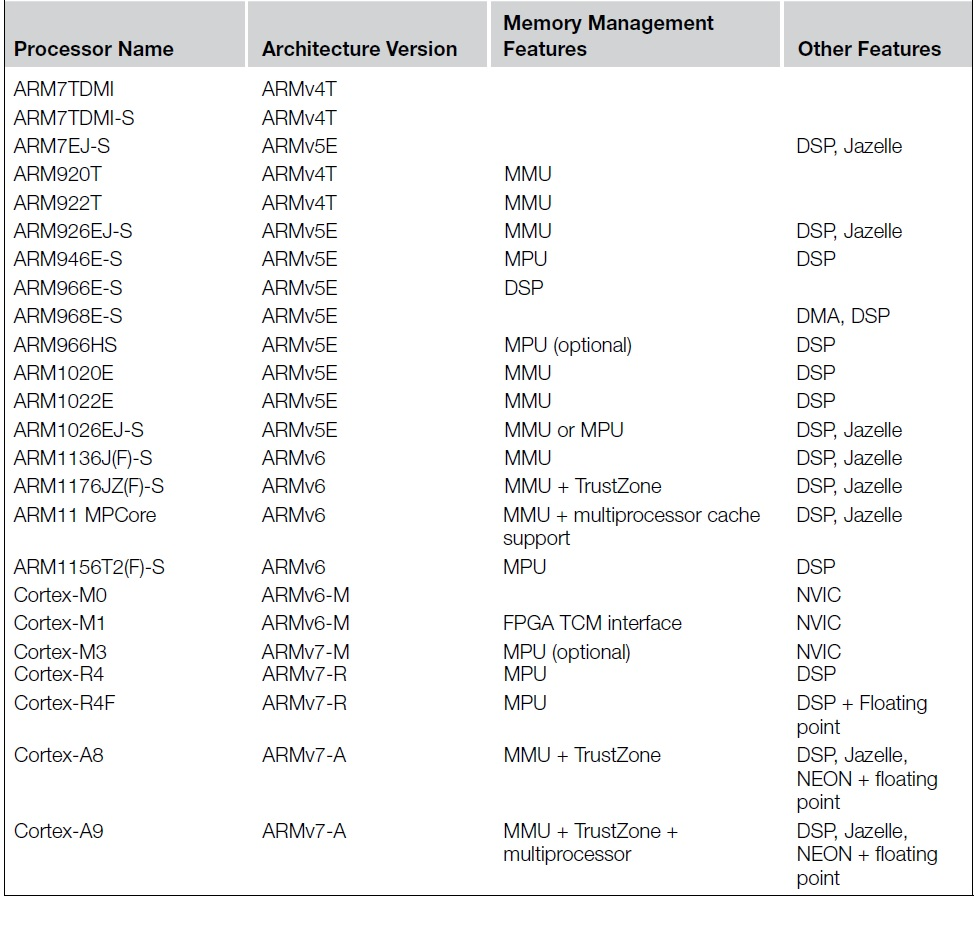
\includegraphics[width=5in]{Nombres.jpg}
\caption{Nombres de los procesadores ARM}
\label{fig2}
\end{figure}

\section{La filosofía de diseño RISC}

El núcleo ARM utiliza una arquitectura RISC. RISC es una filosofía de diseño que busca entregar instrucciones simples pero de gran alcance que se ejecutan dentro de un solo ciclo a una alta velocidad de reloj. La filosofía RISC se concentra en la reducción de la complejidad de las instrucciones realizadas por el Hardware debido a que es más fácil proporcionar gran flexibilidad e inteligencia en software que en hardware. Como resultado, el diseño RISC realiza una gran demanda en el compilador. En contraste, las computadoras tradicionales con conjunto de instrucciones complejas (CISC)depende mas del hardware para la funcionalidad de las instrucciones, y en consecuencia las instrucciones CISC son mas complicadas. En la figura \ref{fig3} se muestran estas diferencias.


\begin{figure}
\centering
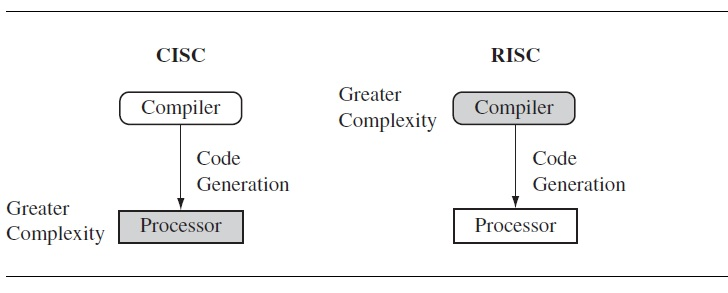
\includegraphics[width=5in]{CISC_RISC.jpg}
\caption{CISC vs. RISC}
\label{fig3}
\end{figure}

La filosofía RISC es implementada con cuatro grandes reglas de diseño:

\begin{itemize}
\item Instrucciones.- El procesador RISC tiene un reducido número de clases de instrucciones. Estas clases proporcionan operaciones simples que pueden ejecutarse en un solo ciclo. El compilador o programador sintetiza operaciones complicadas combinando varias instrucciones simples. Cada instrucciones tiene un tamaño fijo para permitir al pipeline buscar instrucciones futuras antes de decodificar la instrucción actual. En contraste, en los procesadores CISC la instrucciones son comúnmente de tamaño variable y toma muchos ciclos ejecutar.
\item Pipelines.- El procesado de las instruciones es roto en pequeñas unidades que pueden ser ejecutadas en paralelo por pipelines. Idealmente el pipeline avanza un paso en cada ciclo de reloj para un máximo rendimiento. Las instrucciones pueden ser decodificadas en una etapa pipeline. No hay necesidad para que una instruccion sea ejecutada por un miniprograma llamado microcodigo como en los procesadores CISC
\item Registros.- Las maquinas RISC tiene un conjunto de registros de propósito general grande. Cualquier registro contiene o datos o direcciones. Los registron atuan como una memoria de almacenamiento local y rápido para todos los datos de procesamiento de operaciones. En contraste, los procesadores CISC tienen registros de propósito específico.
\item Arquitectura de carga-almacenado .- El procesador trabaja con los datos almacenados en los registros. Separar las instrucciones de carga y almacenado transfiere datos entre el banco de registros y la memoria externa. El acceso a memoria es costoso, de tal forma que separar los accesos de memoria desde el procesamiento de datos proporciona una ventaja porque se pueden almacenar datos en el banco de registros múltiples veces sin necesidad de múltiples accesos a memoria. Sin embargo, con el diseño CISC el procesamiento de datos actúan en la memoria directamente.
\end{itemize}

Estas reglas de diseño permiten al los procesadores RISC ser mas simples, y asi el núcleo puede trabajar a frecuencias de reloj más altas. Los procesadores CISC son mas complejos y trabajan a frecuencias de reloj más bajas.

\section{Sistemas de Hardware Embebido}
Los sistemas embebudos pueden controlar muchos diferentes dispositivos, esde pequeños sensores encontrados en las lineas de producción, hasta sistemas de control en tiempo real usados en la NASA para pruebas espaciales. Todos estos dispositivos usan una combinación componentes de software y Hardware. Cada componente is elegido para mejorar la eficiencia, si es aplicable, es diseñado para futuras extensiones y expansiones.


\begin{figure}
\centering
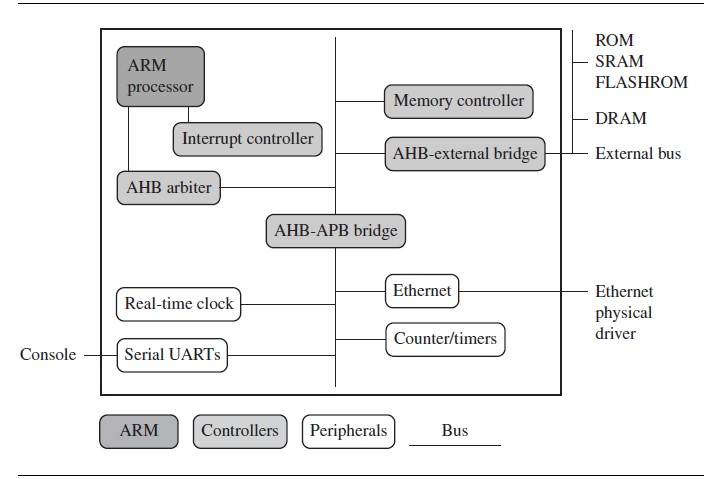
\includegraphics[width=5in]{Microcontroller.jpg}
\caption{Ejemplo de un dispositivo basado en ARM}
\label{fig4}
\end{figure}

La figura \ref{fig4} muestra un dispositivo embebido típico basado en el núcleo ARM. Cada caja representa una característica o función. Las lineas que conectan las cajas son buses que transportan datos. Se pueden separar los dispositivos en cuatro componentes de hardware principales:
\begin{itemize}
\item EL procesador ARM controla un dispositivo embebido. Diferentes versiones de los procesadores ARM estan disponibles para ajustarse a las características de operación deseadas. Un procesador ARM incluye un núcleo ( la máquina de ejecución que procesa las instrucciones y manipula los datos) mas los componentes periféricos que realizan la interfaz con el bus. Estos componentes pueden incluir manejadores de memorias y caches.

\item Los Controladores coordinan bloques importantes funcionales del sistema. Dos bloques de controladores comúnmente encontrados son interruptores y memorias.
\item Los periféricos proporcionan todas las capacidades externas de entrada-salida a el chip y son responsables de las particularidades del dispositivo embebido.
\item Un bus es usado para comunicarse entre diferentes partes del dispositivo.
\end{itemize}


\chapter{Diseño Datapath}

\section{Calculando la máxima frecuencia de Reloj}
El propósito de esta sección es encontrar la máxima frecuencia de reloj y ajustar los tiempos de mantener la señal basados en los tiempos de propagación para circuitos con compuertas combinacionales y secuenciales.

\subsection{Retardo de propagación de compuertas}

La métrica más simple de rendimiento de un dispositivo digital es el tiempo de computación. Comúnmente esto se mide en operaciones por segundo y depende del tipo de operaciones. Para procesadores de propósito general, esto puede ser medido en millones de instrucciones por segundo (MIPS). Para procesadores aritméticos, se puede medir en millones de operaciones de punto flotante por segundo (MFLOPS). El tiempo de computación esta basado parte en la velocidad de reloj y parte en el número de ciclos de reloj por operación. 

Una compuerta digital es construida a partir de un arreglo de transistores de tal manera que realiza una operación matemática. Estos transistores son operados como interruptores on/off. Idealmente los transistores pueden cambiar de on a off en un instante, sin embargo, un transistor real tiene un tiempo de transición finito. Un factor determinante en el tiempo de transición de un transistor es su tamaño físico. Los transistores mas pequeños usualmente tienen tiempo de transición mas pequeños que los transistores grandes. En las tecnologías modernas el tamaño de los transistores es cada vez más pequeño por lo que los retardos continúan decrementando. Los transistores modernos pueden realizar la transición excepcionalmente rápidos, pero el retardo de estos aún debe tomarse en cuenta.

El tipo específio de transistor en una compuerta lógica no es importante tanto como su efecto. El retardo de conmutación de los transistores crea un retardo en la compuerta lógica. El retardo de la compuerta lógica se determina por el tiempo en el cual la señal de salida cambia respecto al cambio de la señal de entrada. Este retardo se llama \emph{retardo de propagación} ($t_{pd}$).

\subsubsection{Retardos de entrada simples/Múltiples}

La compuerta mas simple para analizar en retardo de propagación $t_{pd}$ es el inversor. El inversor tiene una entrada y una salida. Mientras la entrada es una lógica alta, la salida esta en lógica baja. Cuando la entrada cambia de alto a bajo, la salida cambiará de bajo a alto despues de cierto retardo. La entrada e la salida del inversor no cambian instantáneamente desde el valor lógico bajo al alto o viceversa. Este tiempo finito de subida o tiempo de bajada se muestran en la figura \ref{fig11}. El punto de $50\%$ en el tiempo de subida o tiempo de bajada es cuando el nivel de voltaje esta a la mitad entre el valor lógico alto y el bajo. La $t_{pd}$ es medido entre el punto del $50\%$ de subida en la entrada y el punto de $50\%$ de caída en la salida.

El $t_{pd}$ puede ser diferente para el tiempo de subida de salida y el tiempo de caída de salida. Si el tiempo de subida en mas largo que el tiempo de caída, entonces el punto del $50\%$ será desplazado, de lo cual se obtiene un resultado mas largo que $t_{pd}$. Dado que los retardos de propagación pueden ser diferentes, cada uno tiene un notación diferente. Cuando la salida esta cambiando de alto a bajo, el retardo asociado se denomina $t_{phl}$. Cuando la salida esta cambiando de bajo a alto, el retardo asociado se denomina $t_{plh}$. Por simplicidad, el peor caso de los dos retardos de propagación se toma para el tiempo total de la compuerta entera $t_{pd}$.


\begin{figure}
\centering
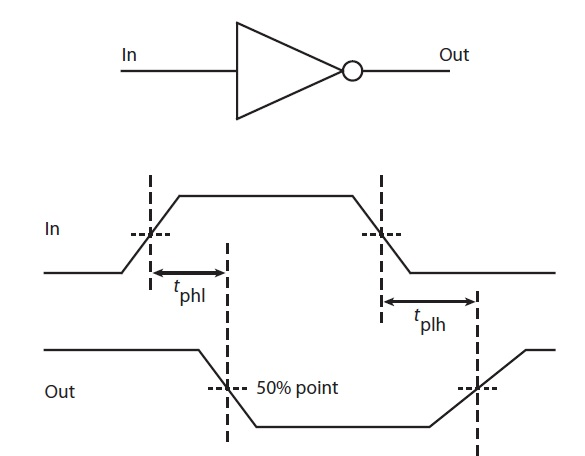
\includegraphics[width=4in]{InverterDelay.jpg}
\caption{Tiempo de propagación de un inversor}
\label{fig11}
\end{figure}

Aún cuando cada tipo de compuerta lógica e construye de manera diferente, el retardo a través de las compuertas es medido de la misma manera. Una compuerta con entradas múltiples tiene muchos retardos de propagación. Por ejemplo, una compuerta AND tiene al menos dos entradas como se muestra en la figura \ref{fig12}. El $t_{pd}$ debe ser medido de bajo a alto y de alto a bajo para cada entrada.

\begin{figure}
\centering
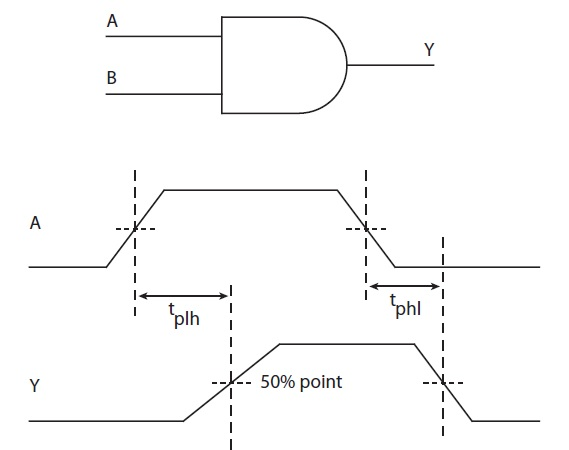
\includegraphics[width=4in]{Anddelay.jpg}
\caption{Retardo de propagación de una Compuerta AND}
\label{fig12}
\end{figure}


Para una compuerta de dos entradas, cuatro retardos de propagación se utilizan: $A2Y_{t_{plh}}$, $A2Y_{t_{phl}}$, $B2Y_{t_{plh}}$, $B2Y_{t_{phl}}$. Para simplificar, se toma el peor caso de los cuatro retardos de propagación y se considera el total $t_{pd}$ para la compuerta entera ($Y_{t_{pd}}$). Esto es cierto para una compuerta combinacional de cualquier número de entradas.  Típicamente, los \emph{datasheet} para los dispositivos lógicos indican el pero caso y el caso típico para $t_{pd}$.



\backmatter
\end{document}
